%!TEX TS-program = xelatex
%!TEX encoding = UTF-8 Unicode
\documentclass[12pt, xcolor=dvipsnames]{beamer}
\definecolor{slight}{gray}{0.9}
\fboxsep=10pt
\usecolortheme[named=Royal Blue]{structure}
\useinnertheme{circles}
\usepackage[no-math]{fontspec}
\usepackage{xltxtra, xunicode}
\usepackage[utf8]{inputenc}
%\usepackage[sc, osf]{mathpazo}
\usepackage[minionint, lf, mathtabular]{MinionPro}
\setmainfont[Mapping=tex-text]{Minion Web Pro}
\setsansfont[Mapping=tex-text]{Myriad Web Pro}
\setmonofont[Scale=MatchLowercase]{Source Code Pro}
\usefonttheme{professionalfonts}
%% 中文字配置
\usepackage[
CJKmath=true, indentfirst=false, PunctStyle={quanjiao},
CheckSingle=true, SlantFont, BoldFont
]{xeCJK}
\setCJKmainfont[Scale=0.9, BoldFont=Hiragino Mincho ProN W6]{Hiragino Mincho ProN W3}
%\setCJKmainfont[Scale=0.9, BoldFont=Noto Sans CJK JP Bold]{Noto Sans CJK JP Medium}
\setCJKsansfont[Scale=0.9, BoldFont=Hiragino Sans W6]{Hiragino Sans W4}
%\setCJKsansfont[Scale=0.9, BoldFont=Hiragino Sans CNS W6]{Hiragino Sans CNS W3}
%\setCJKsansfont[Scale=0.9, BoldFont=Hiragino Sans W7]{Hiragino Sans W4}
%\setCJKsansfont[Scale=0.9, BoldFont=Source Han Sans UI TC Bold]{Source Han Sans UI TC Regular}
%\setCJKsansfont[Scale=0.9, BoldFont=PingFang TC Semibold]{PingFang TC Regular}
\setCJKmonofont[Scale=0.9, BoldFont=Yuanti TC Regular]{Hiragino Maru Gothic ProN W4}
\usepackage{fancyvrb, attachfile2, pstricks}
\usepackage{graphicx}
\setbeamerfont{page number in head/foot}{size=\tiny}
\setbeamertemplate{footline}[frame number]
\usepackage{xmpmulti, booktabs, multicol}
\setbeamertemplate{navigation symbols}{}
\let\WriteBookmarks\relax
\usepackage{dcolumn}
\newcolumntype{.}[1]{D{.}{.}{#1}}
\newcolumntype{,}[1]{D{,}{,}{#1}}

\linespread{1.25}

\setbeamersize{text margin left=.8em, text margin right=.6em}

\makeatletter
\defbeamertemplate{itemize item}{mycircle}{\LARGE\raise-1.6pt\hbox{\textbullet}}
\makeatother

\setbeamertemplate{itemize item}[mycircle]
\setbeamertemplate{itemize subitem}[triangle]
\setlength\leftmargini{1.3em}
\setlength\leftmarginii{1em}


%\CTXFR
\title{\bf{\Huge {}\\[-2mm] Principles of Economics \\[2mm] Review Session}}
\author{{\Large 張耕齊\\[2mm] Keng-Chi Chang}}
\institute{{}\\[-7mm]\footnotesize\tt{<r03323070@ntu.edu.tw>}\\[2mm]}
\date{\large 2016.11.30}
\begin{document}
\fontsize{12}{14pt}\selectfont

\begin{frame}
\titlepage
\end{frame}



\begin{frame}
\frametitle{\bf Foreign \& Domestic Labor Market}
\small \textsf{\bfseries Final 2008 Essay A.} 
Suppose highly educated workers from country Daiwan can participate in two labor markets:
the domestic market and the foreign worker market in BeeKok. Foreign workers who work
at BeeKok are covered by a binding minimum wage law, but domestic workers are not.
\begin{enumerate}\itemsep-0.5ex
\item[1.] Draw a diagram for each of these markets. Is the binding minimum wage higher or lower than the equilibrium wage of the domestic market? Is there a shortage or surplus in the foreign worker market in BeeKok?
\item[2.] If you were a Daiwan worker, what is the maximum you are willing to pay to get a chance to work in BeeKok? Indicate with segments on your graphs.
\end{enumerate}
\end{frame}

\begin{frame}
\small 
\begin{enumerate}\itemsep-0.5ex 
\item[3.] Suppose there is a quota of foreign workers, and there is only one middleman company who can apply for Daiwan workers to work in BeeKok, how much would this company be charging the workers who want to apply? How much would the Daiwan workers be actually earning (net pay)?
\item[4.] Suppose the BeeKok government lowers the minimum wage for foreign workers in BeeKok. Indicate on your graphs how
\begin{enumerate}\itemsep-0.5ex 
\item[i.] actual wages earned (net pay) in both markets,
\item[ii.] the number of Daiwan workers in BeeKok,
\item[iii.] the amount charged by the monopoly middleman company, would change.
\end{enumerate}
Would the shortage or surplus in BeeKok's foreign worker market increase or decrease? Who will be happy about this policy? Will anyone be unhappy with this policy? Explain.
\end{enumerate}
\end{frame}

\begin{frame}
\small 
\begin{enumerate}\itemsep-0.5ex 
\item[5.] How much would the middleman company charge if the minimum wage drops to
zero (non-binding)?
\item[6.] The BeeKok government wants to increase the welfare of foreign Daiwanese
workers in BeeKok. Would you suggest raising or lowering the minimum wage? Why?
\end{enumerate}
\end{frame}



\begin{frame}
\frametitle{\bf Labor Demand}
\small \textsf{\bfseries Final 2008 Multiple Choice Q10.} 
Consider the labor market for heath care workers, which is in equilibrium. Because of the
aging population in the United States, the output price for health care services has increased.
Holding all else equal, what effect does this have on the labor market for health care
employees?\begin{enumerate}\itemsep-0.5ex 
\item[A.] The equilibrium wage increases, and the equilibrium quantity of labor increases.
\item[B.] The equilibrium wage increases, and the equilibrium quantity of labor decreases.
\item[C.] The equilibrium wage decreases, and the equilibrium quantity of labor increases.
\item[D.] The equilibrium wage decreases, and the equilibrium quantity of labor decreases. 
\end{enumerate}
\end{frame}


\begin{frame}
\frametitle{\bf Inequality}
\small \textsf{\bfseries Final 2008 Multiple Choice Q13.} 
Why is a plumber never likely to be as rich as a movie star?
\begin{enumerate}\itemsep-0.5ex 
\item[A.] Compensating differential creates a higher wage in the movie business.
\item[B.] There haven't been any significant technological advances in the plumbing industry.
\item[C.] Productivity levels are low in the plumbing industry due to low worker morale.
\item[D.] A plumber can provide his services to only a limited number of customers. 
\end{enumerate}
\end{frame}



\begin{frame}
\frametitle{\bf §12.1--12.4 Monopoly}
\begin{itemize}
\item Under perfect competition:
\begin{itemize}
	\item There are many buyers and sellers
	\item An individual seller cannot control market price
	\item So they take prices as given and decide the quantities supplied
	\item This is as if they face an horizontal demand curve
	\item An additional quantity sold will earn $P$, and this is by definition $MR$
	\item Maximize profit by choosing quantities such that $MR=P=MC$
\end{itemize}
\item Under monopoly:
\begin{itemize}
	\item There is only one seller, so she can decide the price
	\item She faces the whole downward-sloping demand curve
	\item Maximize profit by choosing quantity such that $MR=MC$
	\item This quantity supplied will determine the market price
\end{itemize}
\end{itemize}
\end{frame}



\begin{frame}
\frametitle{\bf Monopoly}
\small \textsf{\bfseries Bonus Question (ALL 12-6).} 
Consider a monopolist who faces a linear demand curve $P=24-Q$, where $P$ is the price the monopoly charges, and $Q$ is the quantity consumers purchase. Monopolist's marginal revenue $MR=24-2Q$. If demand is linear then demand and $MR$ have the same intercept but $MR$ has twice the slope. The monopolist produces this good at a constant average and marginal cost of $\$6$.
\begin{enumerate}\itemsep-0.5ex 
\item[a.] Show that the monopolist's profit-maximizing price is $\$15$.
\item[b.] Suppose the government imposes a tax of $T$ dollars per unit on the monopolist, so the monopolist's marginal cost is now $6+T$. Show that the monopolist will pass along half of the tax to its customers, that is, show that the profit-maximizing price is now $15+T/2$. 
\end{enumerate}
\end{frame}




\begin{frame}
\small \textsf{\bfseries 2008 Multiple Choice Q4.} 
When a certain monopoly sets its price at \$8 it sells 64 units. When the monopoly sets its price at \$10 it sells 60 units. The marginal revenue for the firm over this range is
\begin{enumerate}\itemsep-0.5ex 
\item[A.] \$2.
\item[B.] \$8.
\item[C.] \$22.
\item[D.] \$88.
\end{enumerate}
\end{frame}



\begin{frame}
\small \textsf{\bfseries 2009 Multiple Choice Q3.} 
If a monopolist's marginal costs increase by \$1 for all levels of output, then
\begin{enumerate}\itemsep-0.5ex 
\item[A.] the monopoly price will rise by \$1.
\item[B.] the monopoly price will rise by more than \$1.
\item[C.] the monopoly price will rise by less than \$1.
\item[D.] there is no change in the monopoly price and profits fall.
\end{enumerate}
\end{frame}



\begin{frame}
\frametitle{\bf §12.5 Monopoly is Inefficient}
\begin{center}
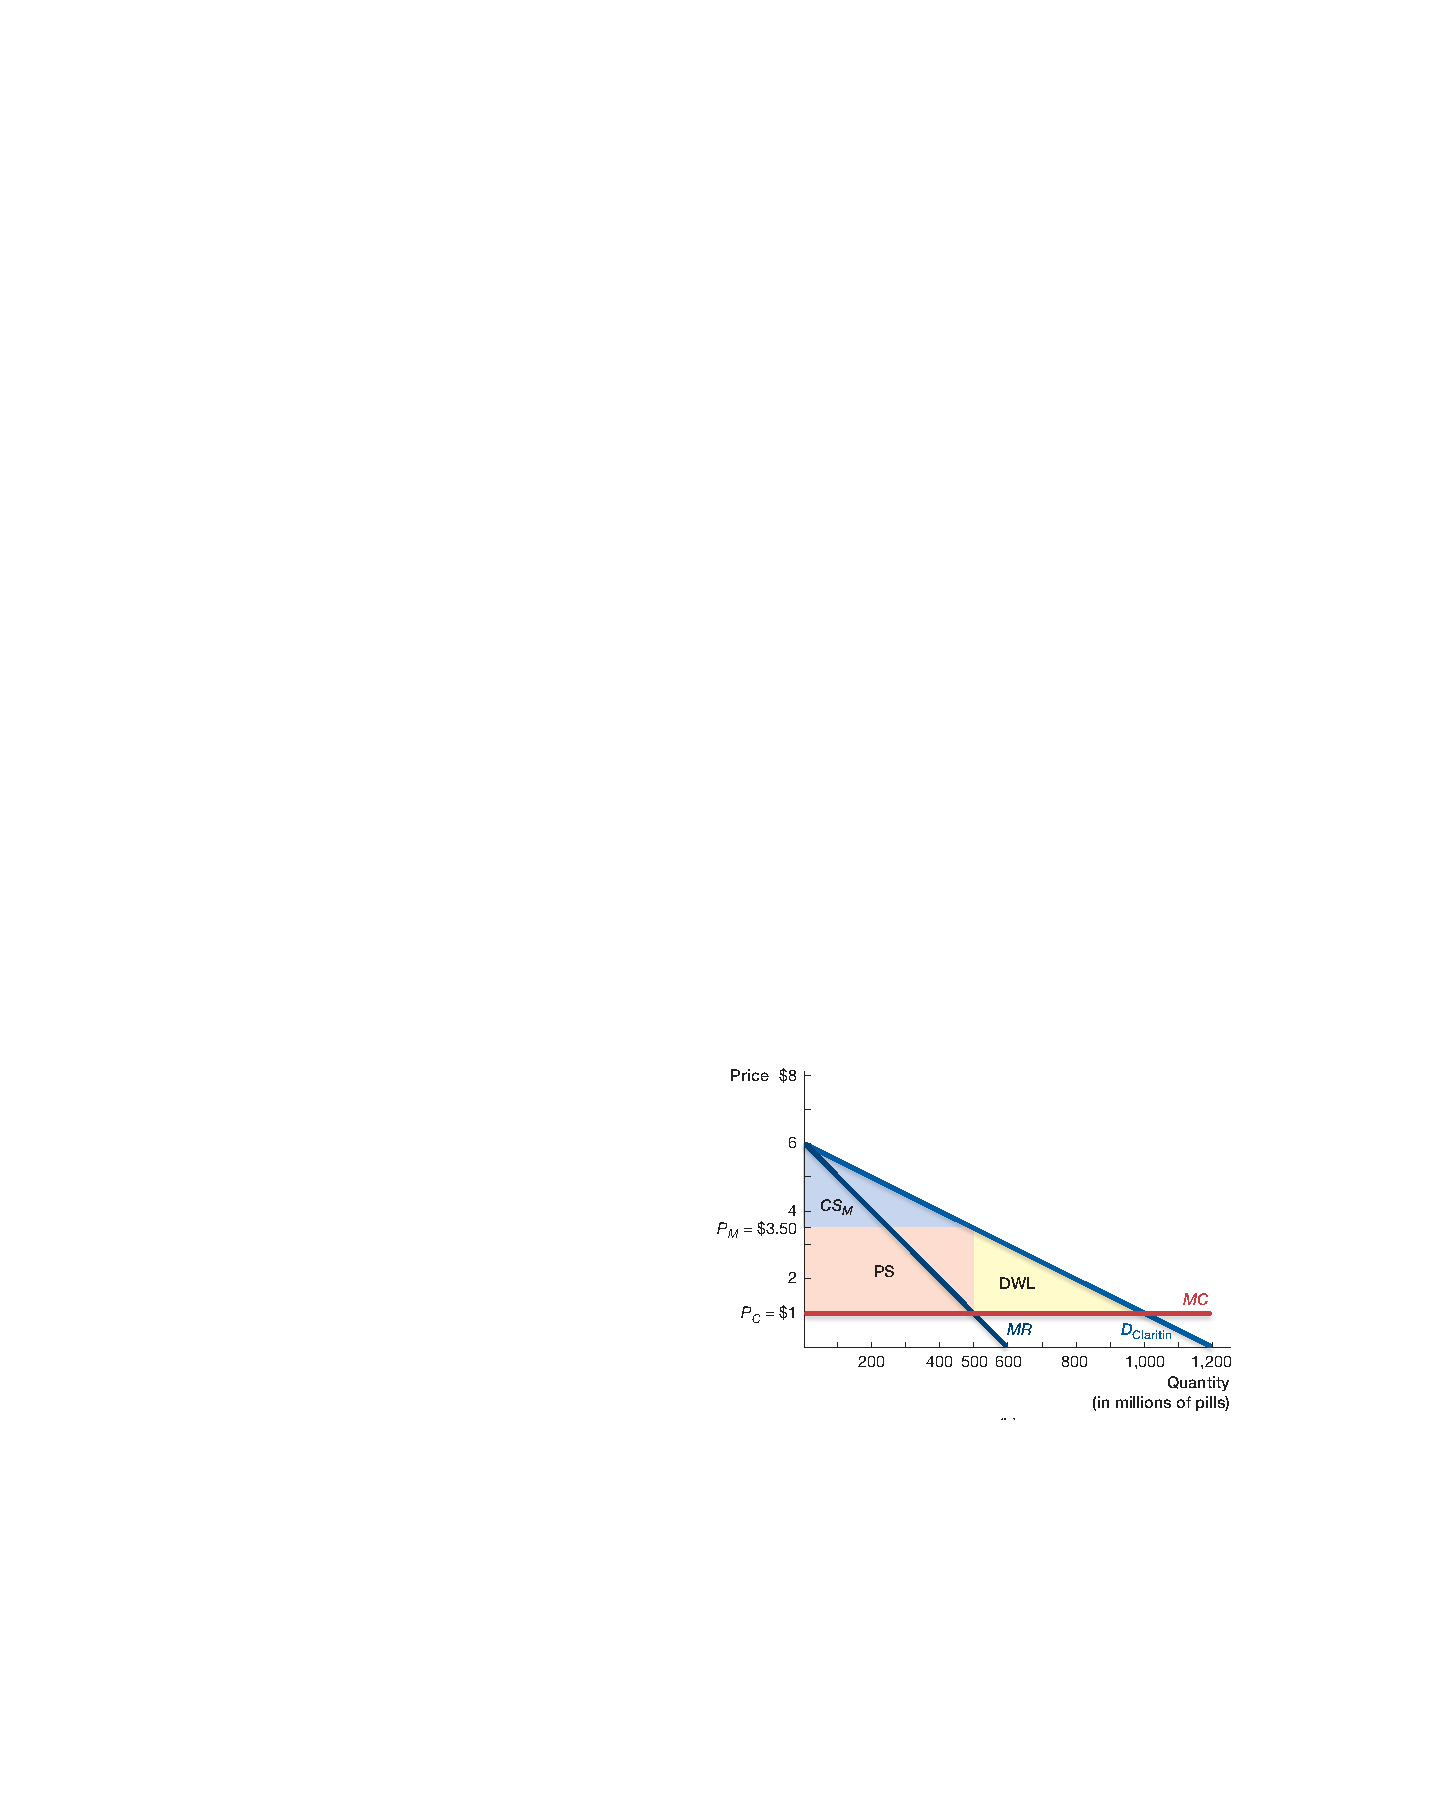
\includegraphics[width=.9\linewidth]{figures/11.pdf}
\end{center}
\end{frame}




\begin{frame}
\frametitle{\bf Monopoly and Efficiency}
\small \textsf{\bfseries ALL 12-12.} 
The annual demand for a new drug HealthyHeart is shown in the diagram below. The one-time cost of developing HealthyHeart is \$2,000. Once the drug has been developed, the marginal cost of an additional pill is \$2.
\begin{center}
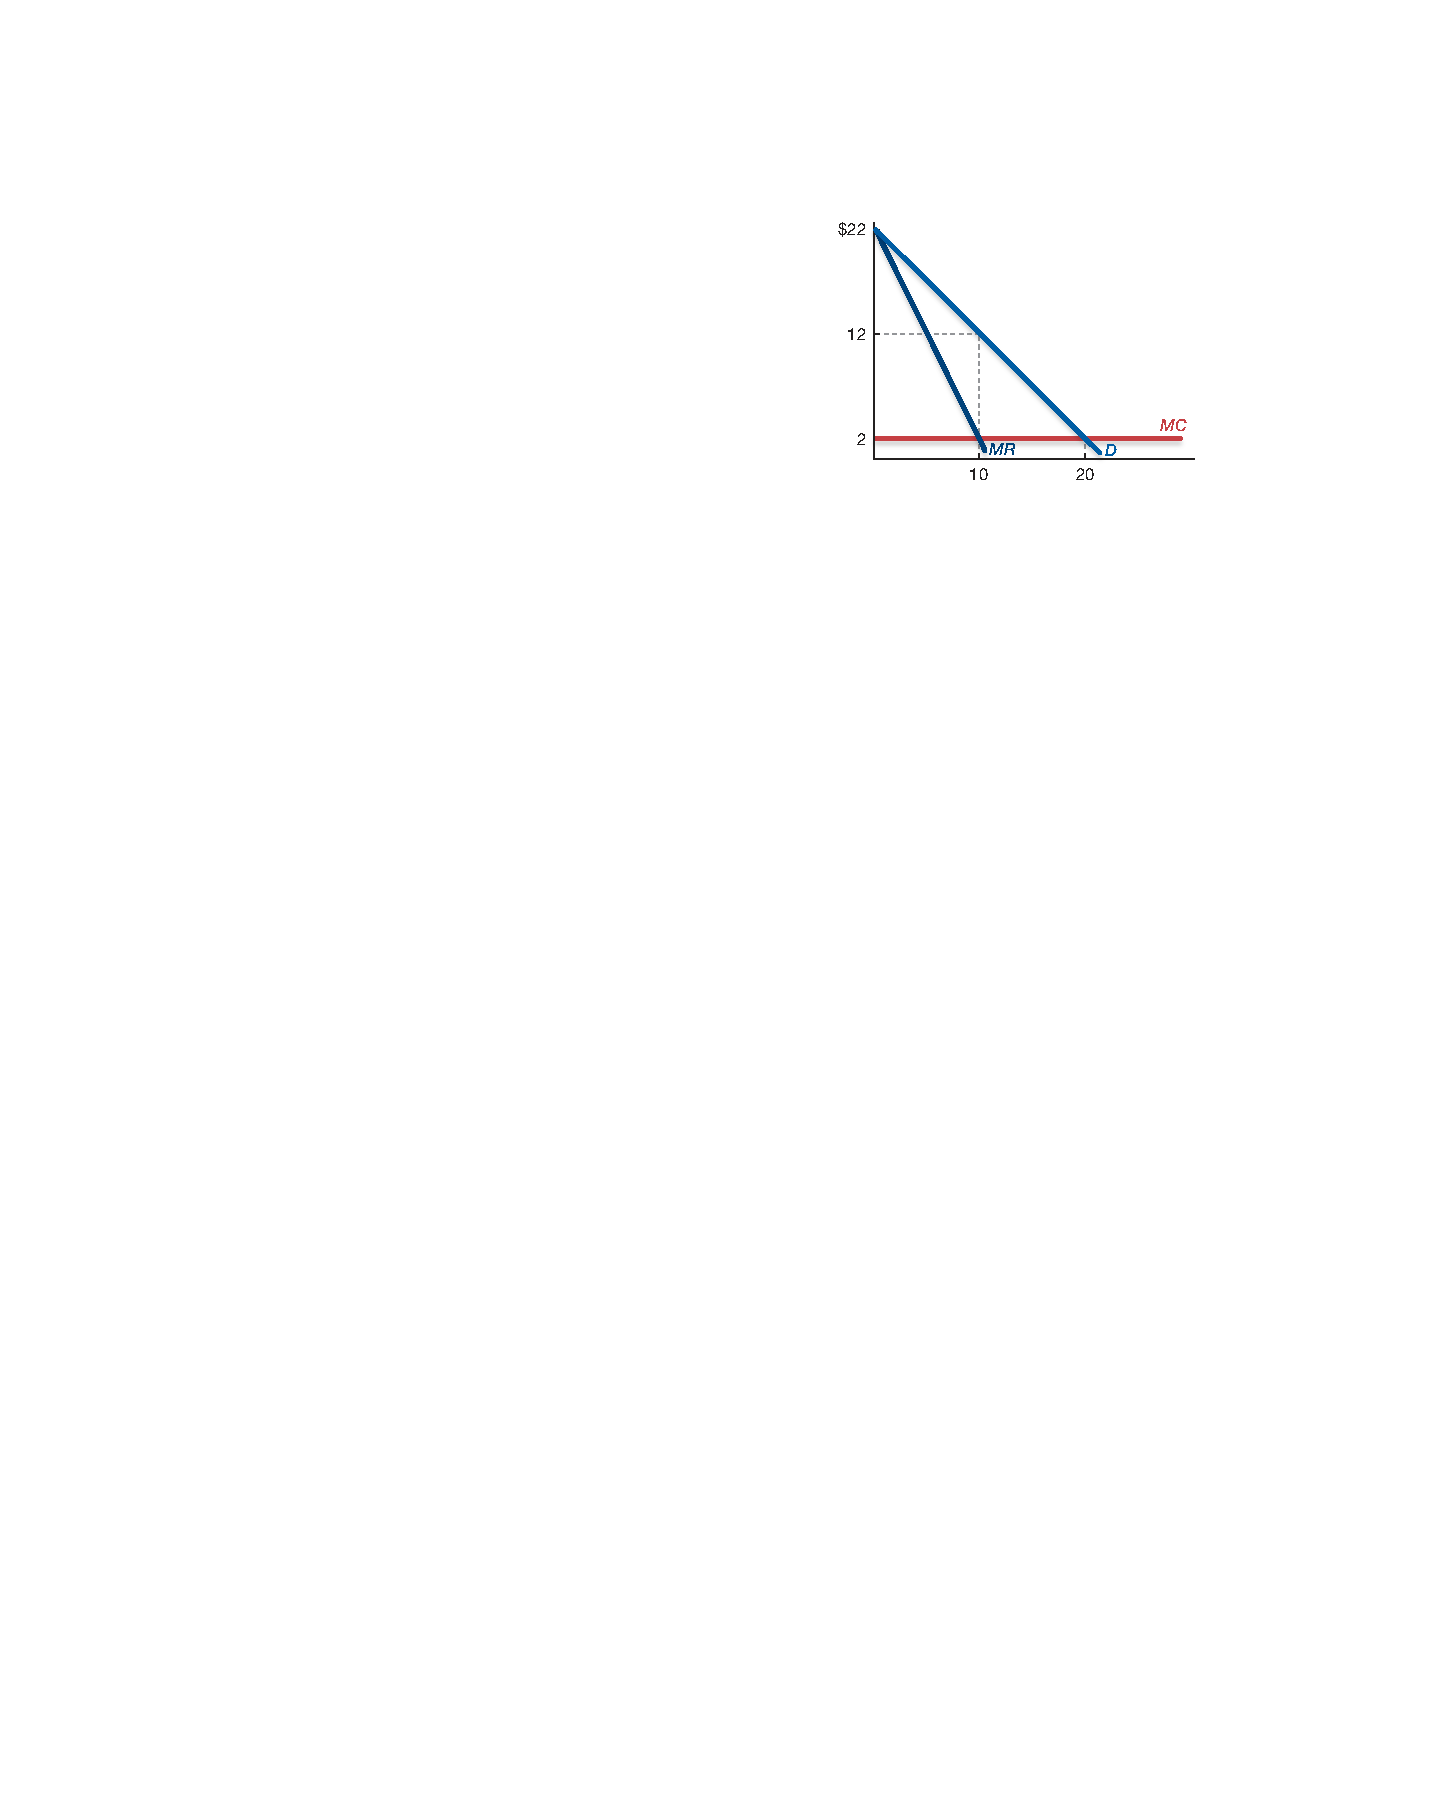
\includegraphics[width=.3\linewidth]{figures/12.pdf}
\end{center}
\begin{enumerate}\itemsep-0.5ex 
\item[a.] Show that if the government gives the company that develops HealthyHeart a 20-year patent the company will be able recover the \$2,000 it spent to develop the drug.
\item[b.] Find the total dead weight loss over the 20-year life of the patent. 
\end{enumerate}
\end{frame}



\end{document}